\section{Initial Experiments}
\subsection{Experimental setup}
In order to validate the spring modeling method, an experiment setup has been constructed as the Figure \ref{fig:Spring_torque_exp_setup} shows. For testing the 50Nm elastic actuator in different poses, the motor is fixed on a adjustable base, so that the inclination of the actuator can be changed. A torque sensor (Lorenz-DF30) is employed to provide a torque ground truth in a range of -50Nm to +50Nm with an accuracy class 0.05\%. Since it's a non-rotary sensor that can only measure the object which does not move, it has been rigidly mounted on the motor and connected to the load through the brakes.
\begin{figure}[htb]
\centering
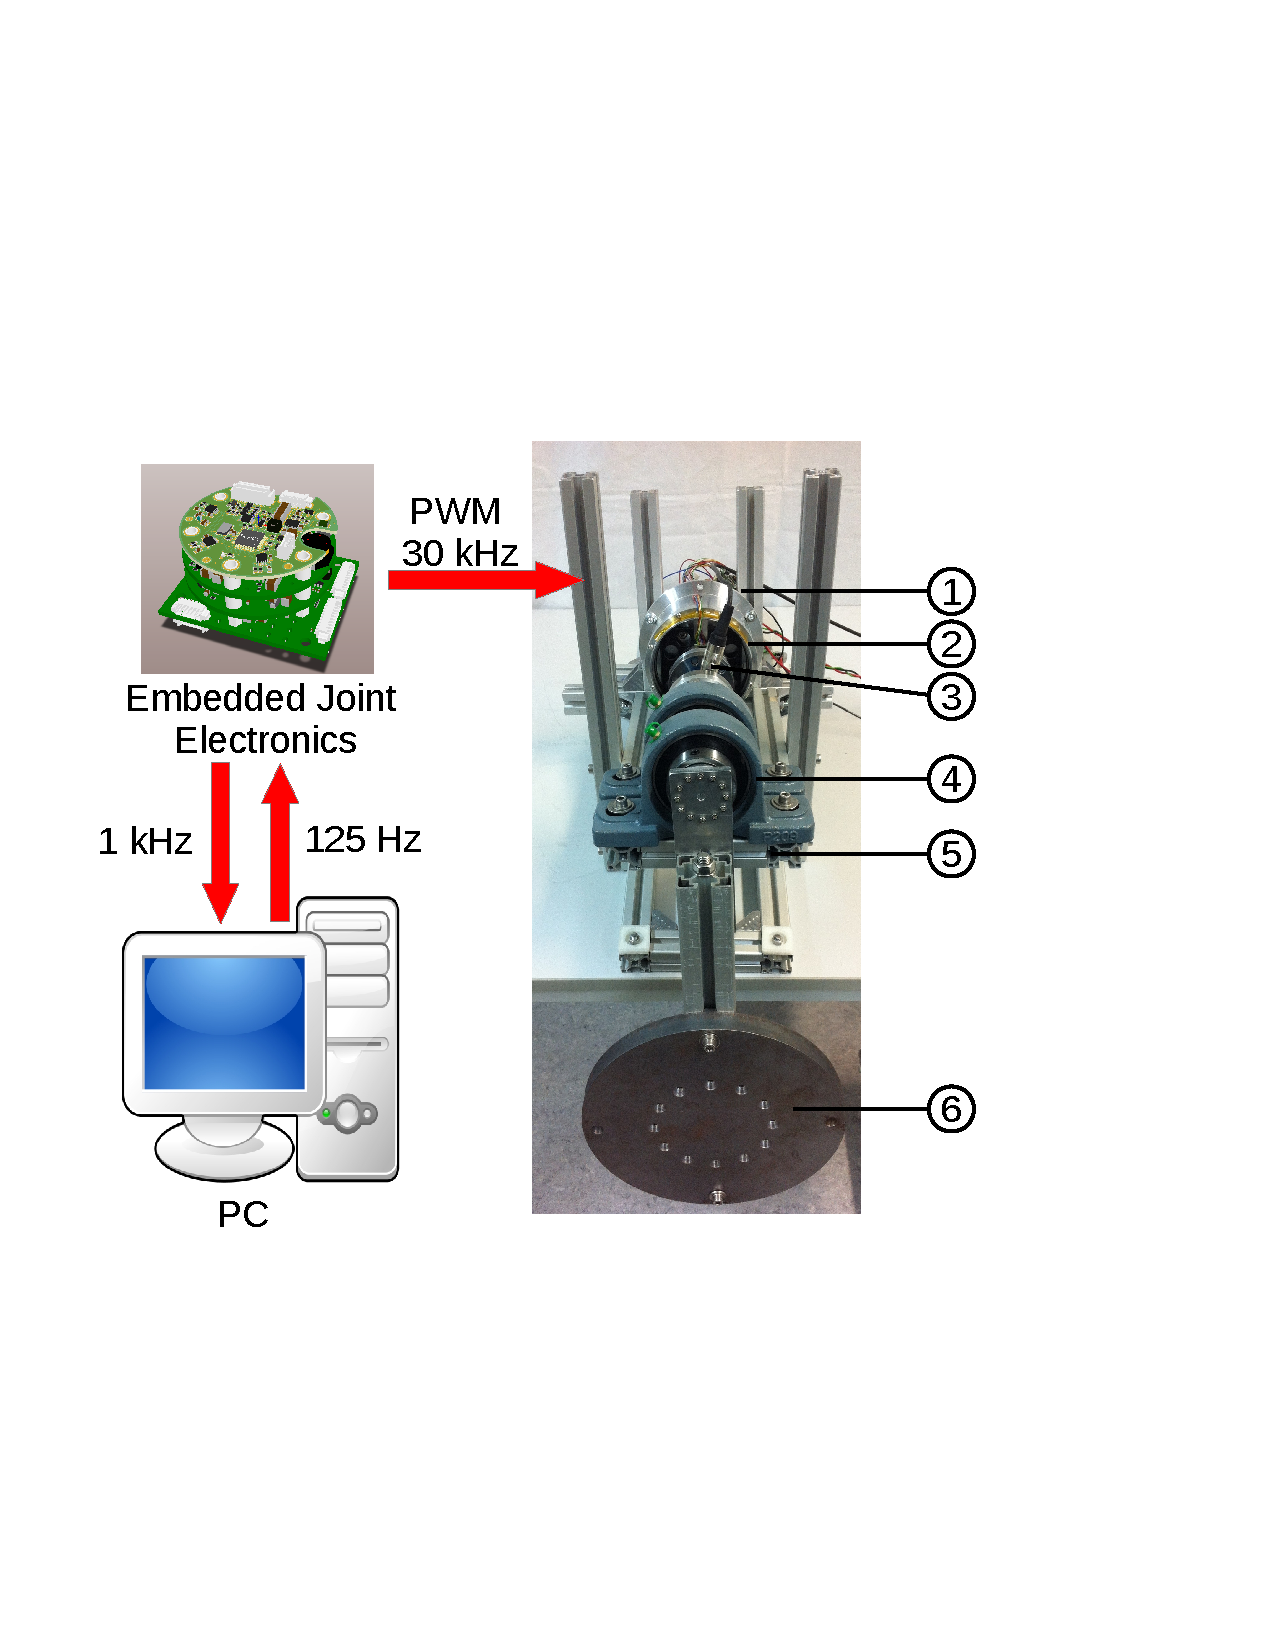
\includegraphics[width=0.8\columnwidth]{./images/4by3_springmodel_testbed.png}
 \caption{Experimental setup used for spring modeling and torque control.}
 \label{fig:Spring_torque_exp_setup}
\end{figure}

\subsection{Spring modeling validation}
The mixture of gaussians are learned from the training data collected using the above-mentioned experimental setup. The training data is gathered by controlling the load to rotate from -170 degree to +170 degree in a position control mode smoothly with a very low speed. The position of the load are changed in each train test and the actuator torque $\tau$, deflection $\delta$, first derivative of deflection $\delta^{\prime}$ and velocity $v$ are measured as the observation variables for the DGMM model $P[\tau,\delta,\delta^{\prime},v]$. At the end of the training procedure, about 1200 mean Gaussians are selected from 6 training tests, which will be used in the next torque control experiment.
%Each entry of the measured variables is compared with the saved variables in the model, when the.. introduce the novelty detection later.

In the testing procedure, the same load is fixed in a random selected position on the lever arm. Based on the trained DGMM model, the actuator torque $\tau$ can be estimated by using conditional probability density function 
\begin{equation}
  %\mathbb{E}[\delta|\tau,\delta^{\prime},v]
    E[\tau|\delta,\delta^{\prime},v] \mbox{ and } V[\tau|\delta,\delta^{\prime},v]
	%E[\delta|\tau,\delta^{\prime},v]
 \label{eq:shape}
\end{equation} 
where $E$ stands for expected value and $V$ stands for expected variance. During testing, the spring deflection is extracted from an embeded deflection sensor, the first derivative of deflection $\delta^{\prime}$ is calculated from the change of the deflection and the time used in a control cycle and the velocity $v$ is acquired from the position sensor. Figure \ref{fig:springmodelcomparison} shows the comparison results between DGMM model $P[\tau,\delta,\delta^{\prime},v]$, $P[\tau,\delta]$ and linear regression model.

%%%%  Figure: evaluation of the model with linear regression model %%%%%
\begin{figure}[htb]
\centering
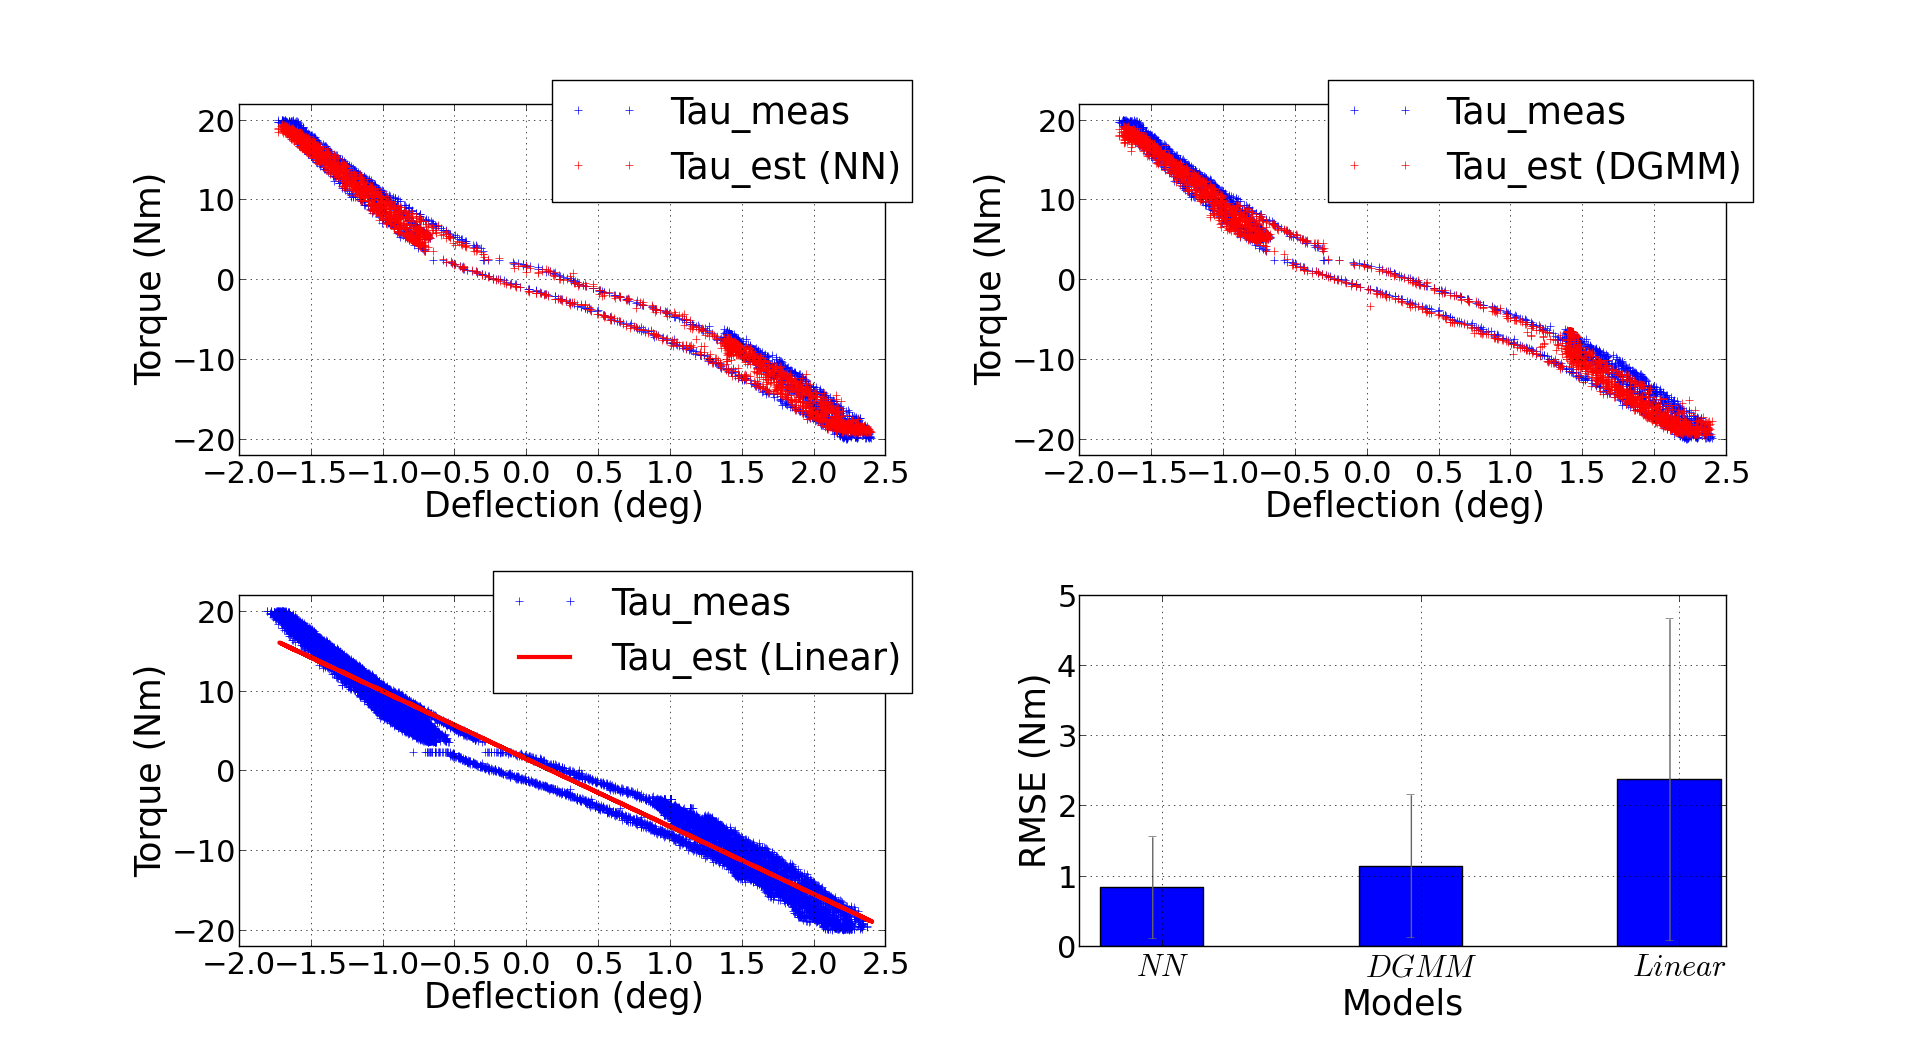
\includegraphics[width=1.1\columnwidth]{./images/4by3_model_comparison.png}
 \caption{\textit{upper left:} measured torque to deflection curves (blue dash line) and corresponding fitted linear line (green line) and estimated torque based on $P[\tau,\delta]$, \textit{upper right:} measured torque to deflection curves (blue line) and estimated torque based on $P[\tau,\delta,\delta^{\prime},v]$ (green dot line), \textit{lower left:} measured torque (blue line) and estimated torque based on $P[\tau,\delta,\delta^{\prime},v]$ (green dot line), \textit{lower right:} root mean squre errors (blue bars) and normalized stardard deviations (black line) of the three models in torque estimation.}
 \label{fig:springmodelcomparison}
\end{figure}

%%%%%%%%%%%%%%%%%%%%%%%%%%%%%%%%%%%%%%%%%%%%%%%%%%%%%%%%%%%%%%%%%%%%%%%

The training data and the testing data are collected by manually moving the load lever arm and the torque is measured by the torque sensor. The DGMM models and the linear regression function are trained from the collected training data, and then they are evaluated by estimating the torque with given input variables in testing data. The RMSE between the estimated torque and measured torque is calculated for each model, as the lower right figure shows, the RMSE of the model $P[\tau,\delta,\delta^{\prime},v]$ is lower than the other two models.

\subsection{Torque control}
For validating the DGMM model $P[\tau,\delta,\delta^{\prime},v]$, the actuator is placed in different inclination angles and the reference sinusoidal input is given in different frequency (means different rotate speed). Figure \ref{fig:torquetracking_model2} shows the results of the validation experiments.
\iffalse
\begin{figure}[htb]
\centering
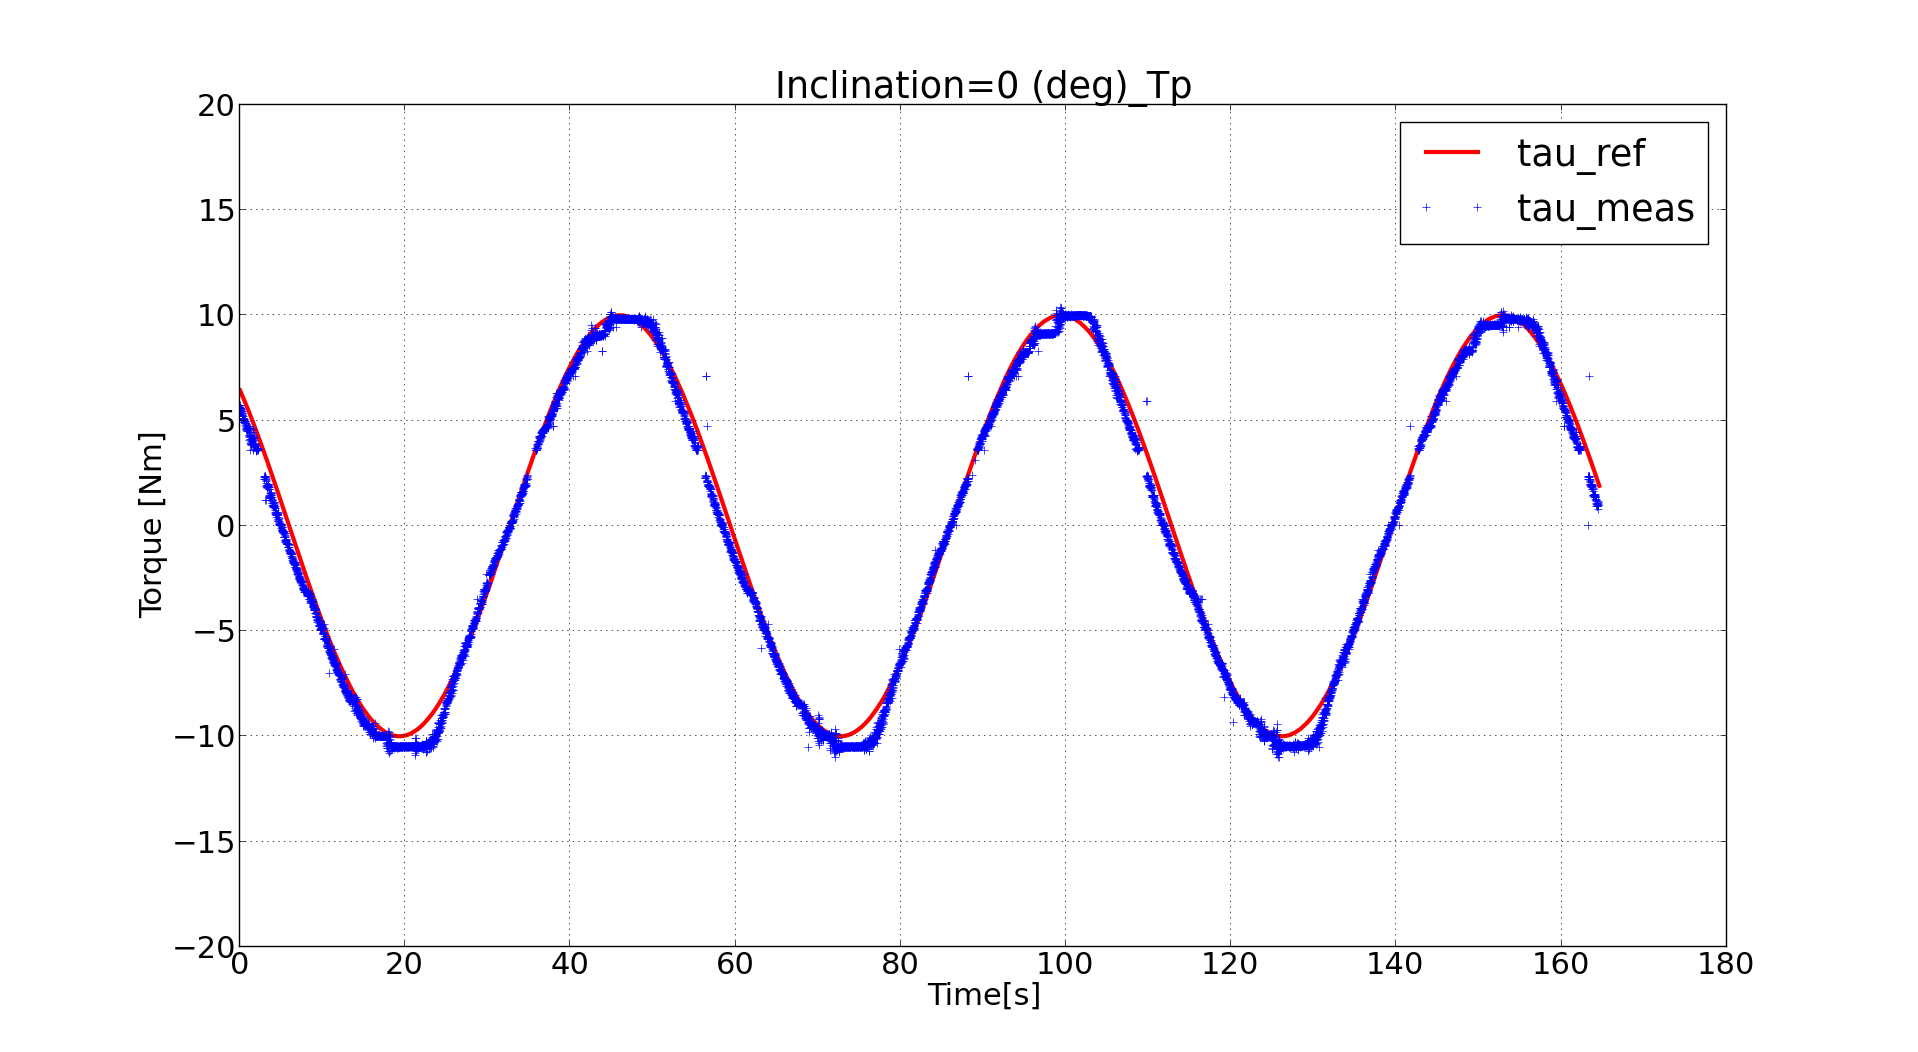
\includegraphics[width=0.8\columnwidth]{./images/4by3_dgmm_ddef_inclination0.png}
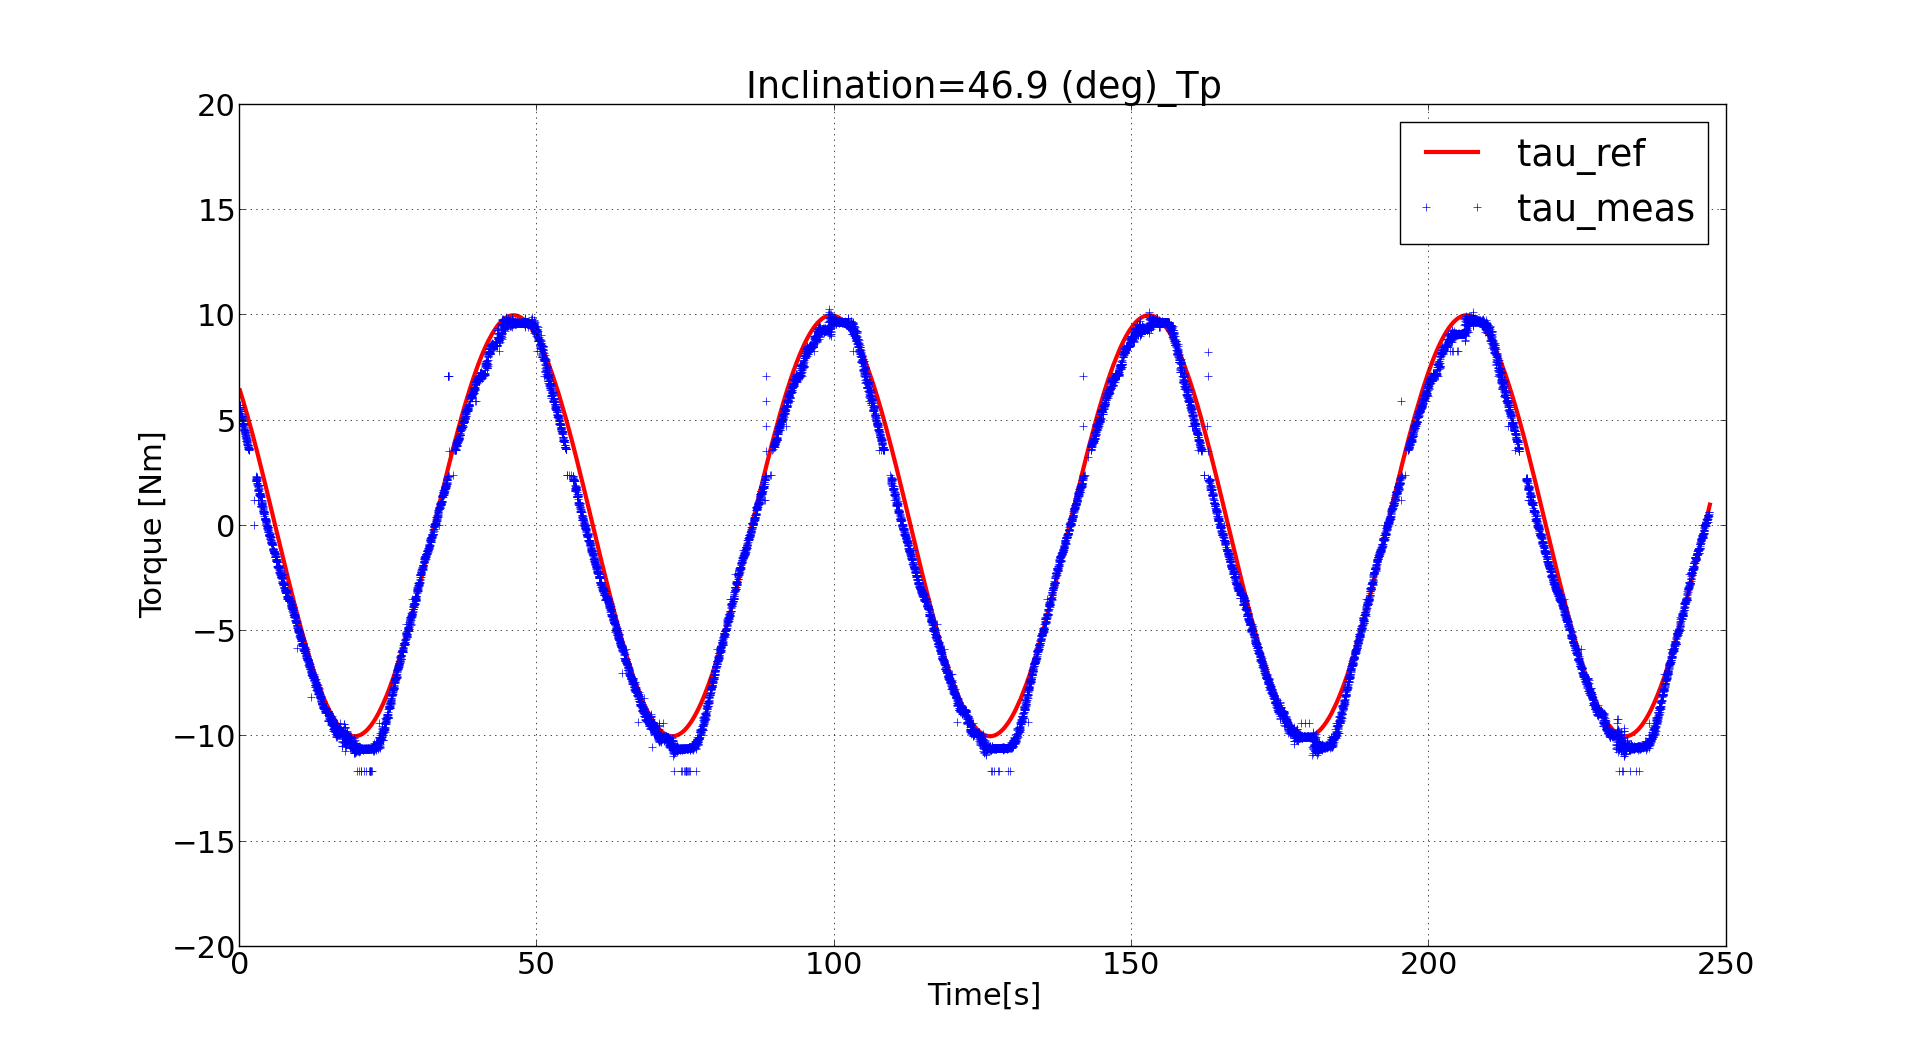
\includegraphics[width=0.8\columnwidth]{./images/4by3_dgmm_ddef_inclination47.png}
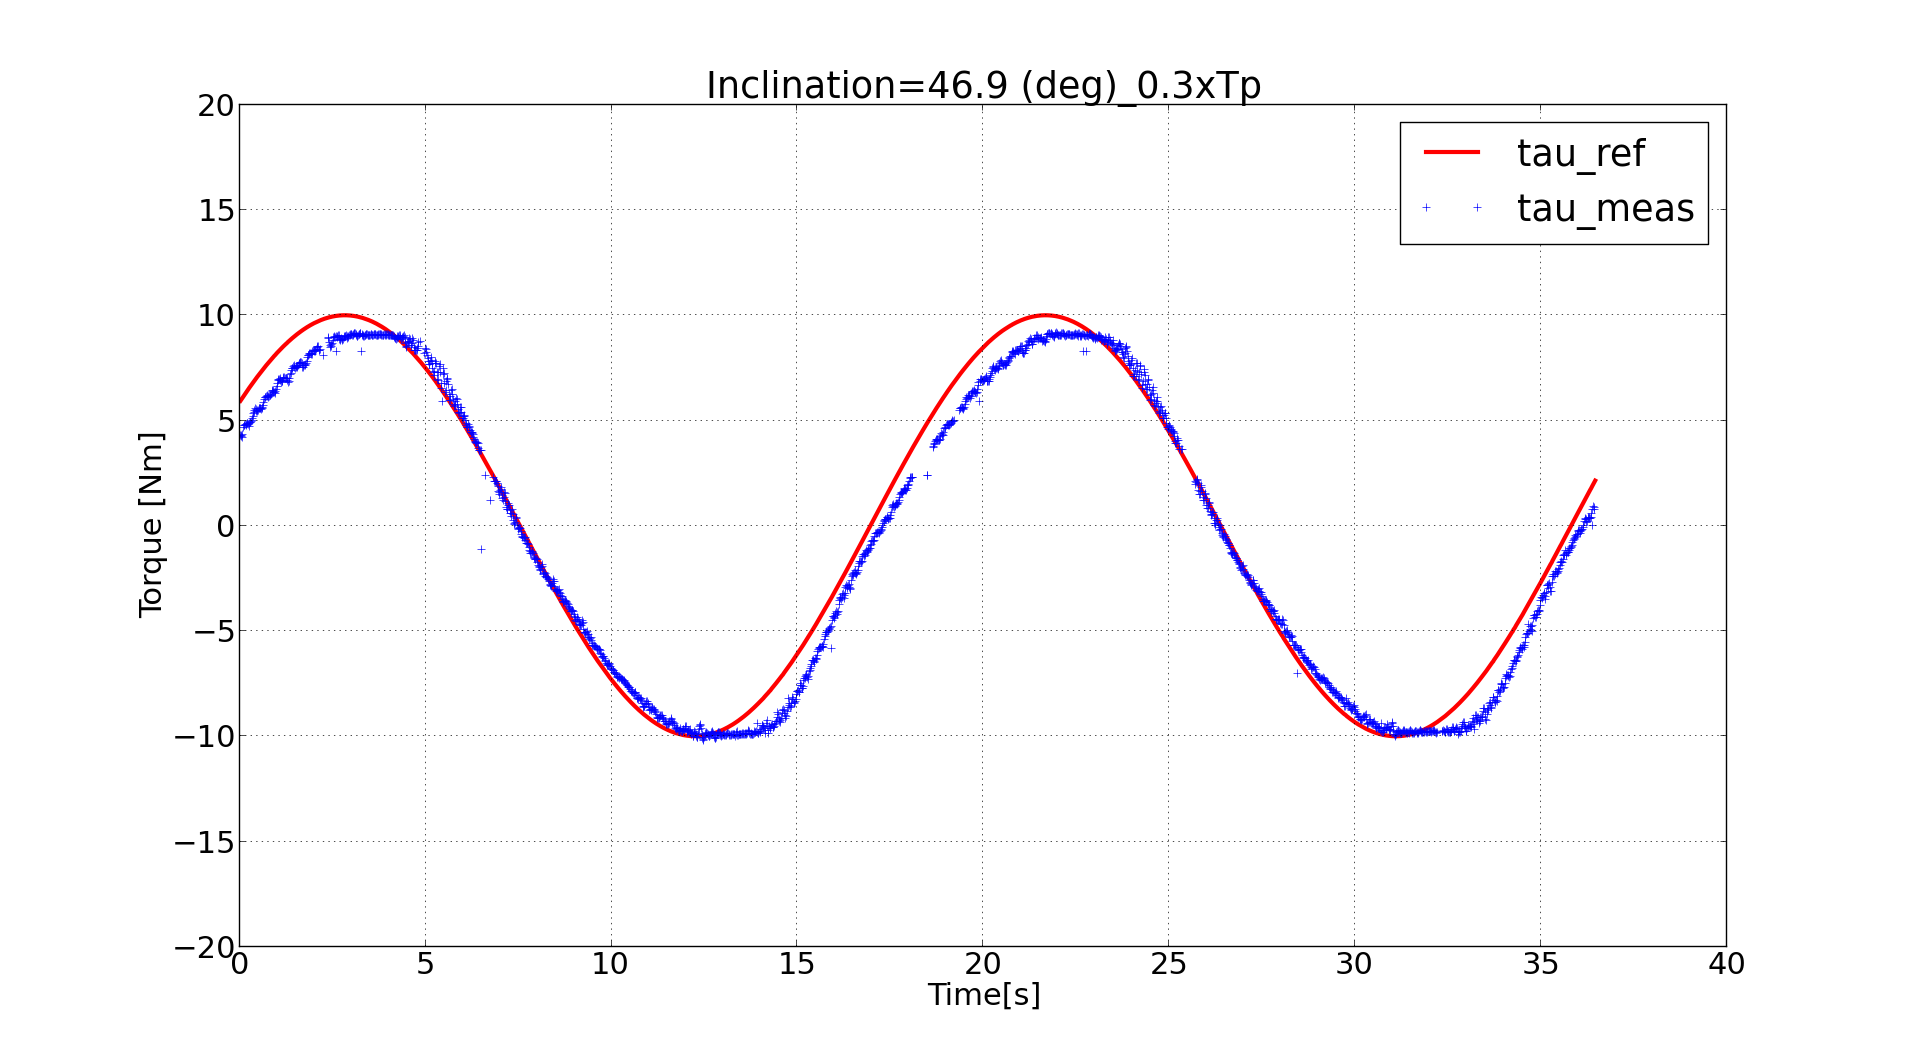
\includegraphics[width=0.8\columnwidth]{./images/4by3_dgmm_ddef_inclination47_3xspeed.png}
 \caption{\textit{upper:} Result of the torque tracking based on DGMM model $P[\tau,\delta,\delta^{\prime},v]$ with testbed inclination equals 0 degree, \textit{middle:} Result of the torque tracking based on DGMM model $P[\tau,\delta,\delta^{\prime},v]$ with testbed inclination equals 46.9 degree, \textit{lower:} Result of the torque tracking based on DGMM model $P[\tau,\delta,\delta^{\prime},v]$ with testbed inclination equals 46.9 degree and higher reference frequency.}
 \label{fig:torquetracking_model2}
\end{figure}
\fi
Comparing upper and middle subfigures, it can be seen that the actuator is still able to track the reference torque finely despite the pose changes. However, when the frequency of the reference input is increased (actuator speed increased), a tracking error can be found when the torque increases from -10 Nm to + 10 Nm. That remains to be further investigated.

%***To evaluate force control performance, both a force-tracking experiment and a zero-force experiment are conducted.\cite{Parietti2011}***
